\iffalse

INSTRUCTIONS: (if this is not lecture1.tex, use the right file name)

  Clip out the ********* INSERT HERE ********* bits below and insert
appropriate TeX code.  Once you are done with your file, run

  ``latex lecture1.tex''

from a UNIX prompt.  If your LaTeX code is clean, the latex will exit
back to a prompt.  Once this is done, run

  ``dvips lecture1.dvi''

which should print your file to the nearest printer.  There will be
residual files called lecture1.log, lecture1.aux, and lecture1.dvi.
All these can be deleted, but do not delete lecture1.tex.
\fi
%
\documentclass[11pt]{article}
\usepackage{amsfonts}
\usepackage{amsmath}
\usepackage{latexsym}
\usepackage{hyperref}
\usepackage{tikz}
\usepackage{tikz-qtree}
\usepackage{pdfpages}
\usepackage{graphics}
\usepackage{graphicx}
\usetikzlibrary{trees}
\usepackage{listings}
\usepackage{array}


\hypersetup{
    colorlinks=true,
    linkcolor=blue,
    filecolor=magenta,      
    urlcolor=cyan,
}
 
\urlstyle{same}

\setlength{\oddsidemargin}{.25in}
\setlength{\evensidemargin}{.25in}
\setlength{\textwidth}{6in}
\setlength{\topmargin}{-0.4in}
\setlength{\textheight}{8.5in}

\newcommand{\handout}[5]{
   %\renewcommand{\thepage}{#1-\arabic{page}}
   \noindent
   \begin{center}
   \framebox{
      \vbox{
    \hbox to 5.78in { {\bf Data Structures and Algorithms} \hfill #2 }
       \vspace{4mm}
       \hbox to 5.78in { {\Large \hfill #5  \hfill} }
       \vspace{2mm}
       \hbox to 5.78in { {\it #3 \hfill #4} }
      }
   }
   \end{center}
   \vspace*{4mm}
}

\newcommand{\lecture}[3]{\handout{L#1}{#2}{}{}{#1}}

\def\squarebox#1{\hbox to #1{\hfill\vbox to #1{\vfill}}}
\def\qed{\hspace*{\fill}
        \vbox{\hrule\hbox{\vrule\squarebox{.667em}\vrule}\hrule}}
\newenvironment{solution}{\begin{trivlist}\item[]{\bf Solution:}}
                      {\qed \end{trivlist}}
\newenvironment{solsketch}{\begin{trivlist}\item[]{\bf Solution Sketch:}}
                      {\qed \end{trivlist}}
\newenvironment{proof}{\begin{trivlist}\item[]{\bf Proof:}}
                      {\qed \end{trivlist}}

\newtheorem{theorem}{Theorem}
\newtheorem{corollary}[theorem]{Corollary}
\newtheorem{lemma}[theorem]{Lemma}
\newtheorem{observation}[theorem]{Observation}
\newtheorem{remark}[theorem]{Remark}
\newtheorem{proposition}[theorem]{Proposition}
\newtheorem{definition}[theorem]{Definition}
\newtheorem{Assertion}[theorem]{Assertion}
\newtheorem{fact}[theorem]{Fact}
\newtheorem{hypothesis}[theorem]{Hypothesis}
%\newtheorem{observation}[theorem]{Observation}
%\newtheorem{proposition}[theorem]{Proposition}
\newtheorem{claim}[theorem]{Claim}
\newtheorem{assumption}[theorem]{Assumption}

%Put more macros here, as needed.
\newcommand{\al}{\alpha}
\newcommand{\Z}{\mathbb Z}
\newcommand{\jac}[2]{\left(\frac{#1}{#2}\right)}
\newcommand{\set}[1]{\{#1\}}

\def\ppt{{\sf PPT}}
\def\poly{{\sf poly}}
\def\negl{{\sf negl}}
\def\owf{{\sf OWF}}
\def\owp{{\sf OWP}}
\def\tdp{{\sf TDP}}
\def\prg{{\sf PRG}}
\def\prf{{\sf PRF}}

%end of macros
\begin{document}

\fbox{
\vbox{
\begin{flushleft}
Ann,  Bob, Charlie    (\emph{replace with your names and correct the date})\\  % authors' names
COSC 336 \\  %class
3/19/2500\\  % date
\end{flushleft}
\center{\Large{\textbf{Assignment 6}}}
} % end vbox
} % end fbox
\vline

\textbf{Instructions.}
\begin{enumerate}
\item Due date and time: As indicated on Blackboard. 
\item This is a team assignment. Work in teams of 3-4 students.  Submit on Blackboard one assignment per team, with the names of all students making the team. 
\item The exercises will not be graded, but you still need to present your best attempt to solve them. If you do not know how to solve an exercise, say it.  This will give me feedback about your understanding of the theoretical concepts.
\item Your programs must be written in Java.

\item Write your programs neatly - imagine yourself grading your program and see if it is easy to read and understand. 

Comment your programs reasonably: there is no need to comment lines like "i++" but do include brief comments describing the main purpose of a specific block of lines.
\item  You will submit on \textbf{Blackboard} 2 files.  

The \textbf{1-st file} is a pdf file (produced ideally with latex and Overleaf) and it will contain the following:
\begin{enumerate}
\item The solution to the Exercises (see the remark above).
\item   A short description of your algorithm for the Programming Task.
\item   A table with the results your program gives  for the data sets indicated for the programming task. 
\item   The java code (so that the grader can make observations) of the  program.
\end{enumerate}


The \textbf{2-nd file} is the .java file containing the java source code for Programming Task.

\end{enumerate}
\newpage










\textbf{Exercise 1.} Consider inserting the keys $10, 22, 31, 4, 15, 28, 17, 88, 59$ into a hash table of length $m=11$ using open addressing with the  hash function $h(x) = x \pmod{11}$ and linear probing, quadratic probing, and double probing. Illustrate  the result by showing the 3 tables obtained  after inserting these keys using 

$\bullet$ linear probing, 

$\bullet$ quadratic probing



$\bullet$ double hashing with $h_1(x) = x \pmod{11} $ and $h_2(x) = 7 - x \pmod{7}$.
  
\textbf{Answer:}
\newline
\newline
\textbf{Linear}
\begin{center}
\begin{tabular}{|c c c |} 
 \hline
 Index & Key & $H_i(x)$ \\ 
 \hline\hline
 0 & 22 &  $H_0(10)$ \\ 
\hline
 1 & 88 & $H_1(88)$ \\ 
 \hline
 2 & - & -  \\ 
 \hline
 3 & - & -  \\ 
 \hline
 4 & 4 & $H_0(4)$  \\ 
 \hline
 5 & 15 & $H_1(15)$  \\
  \hline
6 & 28 & $H_0(28)$  \\ 
 \hline
 7 & 17 & $H_1(17)$  \\ 
 \hline
 8 & 59 & $H_4(59)$   \\ 
 \hline
 9 & 31 & $H_0(31)$  \\
  \hline
10 & 10 & $H_0(10)$  \\
  \hline
\end{tabular}
\end{center}
\begin{verbatim}
    i = 0 : H(10) = (10 + 0) % 11 = 10 
    i = 0 : H(22) = (22 + 0) % 11 = 0 
    i = 0 : H(31) = (31 + 0) % 11 = 9
    i = 0 : H(4) = (4 + 0) % 11 = 4
    i = 0 : H(15) = (15 + 0) % 11 = 4
    i = 1 : H(15) = (4 + 1) % 11 = 5
    i = 0 : H(28) = (28 + 0) % 11 = 6
    i = 0 : H(17) = (17 + 0) % 11 = 6
    i = 1 : H(17) = (6 + 1) % 11 = 7
    ...
    i = 4 : H(88) = (4 + 4) % 11 = 8

    
\end{verbatim}
\pagebreak
\textbf{Quadratic}
\begin{center}
\begin{tabular}{|c c c |} 
 \hline
 Index & Key & $H_i(x)$ \\ 
 \hline\hline
 0 & 22 &  $H_0(10)$ \\ 
\hline
 1 & 88 & $H_1(88)$ \\ 
 \hline
 2 & - & -  \\ 
 \hline
 3 & - & -  \\ 
 \hline
 4 & 4 & $H_0(4)$  \\ 
 \hline
 5 & 15 & $H_1(15)$  \\
  \hline
6 & 28 & $H_0(28)$  \\ 
 \hline
 7 & 17 & $H_1(17)$  \\ 
 \hline
 8 & 59 & $H_2(59)$   \\ 
 \hline
 9 & 31 & $H_0(31)$  \\
  \hline
10 & 10 & $H_0(10)$  \\
  \hline
\end{tabular}
\end{center}
\begin{verbatim}
    hi(X) = (Hash(X) + i^2) % TableSize
    h0(X) = Hash(X) % TableSize
    h1(X) = Hash(X) + 1 % TableSize
    h2(X) = Hash(X) + 4 % TableSize
    h3(X) = Hash(X) + 9 % TableSize

    i = 0^2 , 1^2 , 2^2 , 3^2 , ... 

    all H_0 and H_1 are the same as linear...

    only change H_2(59) = ( 4 + (2^2) ) % 11 = 8 

\end{verbatim}
\bigskip
\textbf{Double hashing}
\begin{center}
\begin{tabular}{|c c c |} 
 \hline
 Index & Key & $H_i(x)$ \\ 
 \hline\hline
 0 &  22 &  $H_0(22)= (22\%11)$ \\ 
\hline
 1 & 88 & $H_4(88)= ( 0+ 4 * 3 )\%11$ \\ 
 \hline
 2 & - & -  \\ 
 \hline
 3 & 17 & $H_2(17)= (6 + 2 * 4)\%11$  \\ 
 \hline
 4 & 4 & $H_0(4)= 4\%11$  \\ 
 \hline
 5 & 15 &  $H_2(15)= (4 + 2*6)\%11$  \\
  \hline
6 &28 &  $H_0(28)=(6+ 0 )\%11$ \\ 
 \hline
 7 & - & -  \\ 
 \hline
 8 & 59 & $H_1(59)= (4 + 1 * 4)\%11$   \\ 
 \hline
 9 & 31 & $H_0(31)= (31\%11 + 0)\%11$ \\
  \hline
10 & 10 & $H_0(10)= (10\%11 + 0)\%11$  \\
  \hline
\end{tabular}
\end{center}
\bigskip
\begin{verbatim}
    Given x = [10, 22, 31, 4, 15, 28, 17, 88, 59]
    H_1(x) = x % 11
    H_2(x) = (7-x) % 7
    
    Note: the chapter PPT uses the following
    H_i(x) = (H_1(x) + (i-1) * H_2(x)) mod 11
    i = 0, 1, 2, 3, 4 ...

     Issue: If we use the PPT formula it combines both H_1(x) and H_2(x) 
            but produces a diffrent H_0(x) and gets stuck on key 28
            (when following the formula from i=0 H_0(x) on all keys).

    We used : H_i(x) = ((H_1(x))+(i)*(H_2(x))) mod 11

    all keys worked but key 28 could present issues if 6 index was taken first as 
    H_2(28) = 0
    7-28 = -21 
    -21 mod 7 = 0
    No incrementing of i will allow for another index to generate...
\end{verbatim}





\textbf{Exercise 2.}  Recall the \textsf{Partition} subroutine employed by \textsf{QuickSort}. You are told that the following array has been partitioned around some pivot element:
\medskip

\begin{tabular}{|c|c|c|c|c|c|c|c|c|}
\hline 
3 & 1& 2 & 4 &5 &8 & 7 & 6 & 9 \\
\hline
\end{tabular}
\medskip

Which of the elements could have been the pivot element? (List all that apply; there could be more than one possibility.)
\medskip

\textbf{Answer:} The elements that could have been the pivot are: \textbf{4, 5, and 9}, as for each of these, all elements to the left of the pivot are less than or equal to it, and all elements to the right are greater.
\bigskip


\textbf{Exercise 3.}
Let $\alpha$ be some constant, independent of the input array length $n$, strictly between $0$ and $1/2$. What is the probability that, with a randomly chosen pivot element, the \textsf{Partition} function produces a split in which the size of both the resulting subproblems is at least $\alpha \cdot n$. Choose the answer from the following list and justify your answer.
\begin{itemize}
\item $\alpha$
\item $1 - \alpha$
\item $1-2\alpha$
\item $2 - 2 \alpha$
\end{itemize}
\medskip

\textbf{Answer:} $1 - 2\alpha$

\textit{Justification:} To ensure both subarrays have size at least $\alpha n$, the pivot must not be among the smallest $\alpha n$ or the largest $\alpha n$ elements. Only the middle $(1 - 2\alpha)n$ elements satisfy this. Since the pivot is chosen uniformly at random, the probability is:
\[
\frac{(1 - 2\alpha)n}{n} = 1 - 2\alpha
\]

\bigskip


\newpage



\textbf{Programming task} The program involves various operations for binary search trees. Your task is to modify the program  at

%\url{https://www.geeksforgeeks.org/binary-search-tree-set-1-search-and-insertion/}

\url{https://www.geeksforgeeks.org/insertion-in-binary-search-tree/?ref=lbp}
\medskip

$\bullet$ Add to the class \textsf{Node}  a data member called \textsf{int size} which keeps the number of nodes in the tree rooted at that node (including in the count the node itself). The constructors and the insertion function need to take into account the sizes of the nodes.
\medskip

$\bullet$ Modify the \textsf{insert} function so that duplicates are also inserted (which is not done in the version at the above link). If the value $x$  to be inserted is equal to the value in the root, insert $x$ in the left subtree.
\medskip





$\bullet$  Write two functions called \textsf{leftRotate (Node t)}, which rotates the root t to the left, so that the right child of t (if there is one; otherwise the rotation does not do anything) becomes the parent of t, and symmetrically  \textsf{rightRotate (Node t) which rotates the root to the right}. See Figure 13.2, page 313 in the textbook, or Notes 6 on Blackboard. Note that when you do \textsf{leftRotate (Node t)}, you need to change the size of \textsf{t} and of \textsf{t.right}, and similarly for \textsf{rightRotate}.


\tikzset{every tree node/.style={minimum width=2em,draw,circle},
         blank/.style={draw=none},
         edge from parent/.style=
         {draw,edge from parent path={(\tikzparentnode) -- (\tikzchildnode)}},
         level distance=1.5cm}
\begin{tikzpicture}
\Tree
[.7     
    [.3 ]
    [.10
    \edge[]; {9}
    \edge[]; [.13
             \edge[]; {11}
             \edge[blank]; \node[blank]{};
         ]
    ]
]
\end{tikzpicture}

For instance for the tree in the figure,  node 7 has size 6, node 3 has size 1, node 9 has size 1, node 10 has size 4, node 13 has size 2, and node 11 has size 1.

If we do \textsf{leftRotate} for the root we get the tree

\begin{tikzpicture}
\Tree
[.10   
    [.7 
    \edge[]; {3}
    \edge[]; {9}
    ]
[.13 \edge[]; {11}
\edge[blank]; \node[blank]{};]
]
\end{tikzpicture}

To test the augmented class, you will insert some values and then do a \emph{preorder} traversals and print in this order  the pairs (value, size) of all the nodes. 	Next, you \textsf{leftRotate} the root and print again the tree after rotation. In other words, you do a preorder traversal \textbf{before and after} the rotation, but print the elements in this order.

\textbf{Test data 1:} insert 7, 10, 3, 9, 13, 11. Your program will print: (7,6), (3,1), (10,4), (9,1), (13, 2), (11,1).
Next, do a \textsf{leftRotate}, and print the tree after rotation and you get (10,6), (7,3), (3,1), (9,1) (13,2), (11, 1).




\textbf{Test data 2:}  Insert one by one the numbers in the file input-6.1. The first line contains how many numbers are there (there are 1000 numbers), and the next line contains the list of numbers.

Report in the pdf file the first 25 pairs (you do complete preorder traversals before and after but report only the first 25 elements).

\textbf{Test data 3:} Insert one by one the numbers in the file input-6.2. The first line contains how many numbers are there (there are 10000 numbers), and the next line contains the list of numbers.

Report in the pdf file the first 25 pairs (as above).

\pagebreak
\section*{Code Description}
    We are tasked with adding a size member to each node that will hold the number of nodes in the subtree rooted at a given node (including node itself). This is accomplished by adding an integer size member that is initilized to 1 when a new node is constructed. During insertion and rotation the size must also be corrected which is done by setting a given nodes size to  $1 + \text{Size}_\text{Right Subtree} + \text{Size}_\text{Left Subtree}$

\begin{center}
    \begin{tikzpicture}[sibling distance=1.5cm, level distance=1.5cm,
      every node/.style = {shape=circle, draw, align=center}]
    \node[draw=none, shape=rectangle] at (0,1) {Before Left Rotation};
    \node {x}
      child {node {C}}
      child {node {y}
        child {node {A}}
        child {node {B}}
      };
    \end{tikzpicture}
\hspace{2cm}
    \begin{tikzpicture}[sibling distance=1.5cm, level distance=1.5cm,
      every node/.style = {shape=circle, draw, align=center}]
    \node[draw=none, shape=rectangle] at (0,1) {Tree 2 (After Left Rotation};
    \node {y}
      child {node {x}
        child {node {C}}
        child {node {A}}
      }
      child {node {B}};
    \end{tikzpicture}

\end{center}

    Rotation is accomplished through a refactoring as seen above. The algorithm for leftRotate for example, first creates a pointer to \textit{y} and \textit{A}. We then assign \textit{y} as the new root by attaching the current root, \textit{x}, to its left link. We then restore the tree by assigning \textit{A} as the old root's right child. The function returns a pointer to the new root \textit{y}. This completes the rotation while still preserving the BST properties. After the rotation is complete size is adjusted as explained above. \\
    \textit{NOTE}: rotateRight works in the exact way but mirrored.

\pagebreak

\section*{Output}
\begin{center}
\begin{tabular}{|p{10em}|p{30em}|} 
\hline
\textbf{Input} & \textbf{Output} \\ 
\hline
[7, 10, 3, 9, 13, 11] & Before rotation: (7, 6) (3, 1) (10, 4) (9, 1) (13, 2) (11, 1) \newline After left rotation: (10, 6) (7, 3) (3, 1) (9, 1) (13, 2) (11, 1) \\ 
\hline 
input-6-1.txt & Before rotation: (448, 1000) (184, 447) (43, 187) (10, 43) (4, 8) (0, 4) (3, 3) (1, 1) (4, 1) (9, 3) (5, 2) (8, 1) (32, 34) (23, 23) (11, 12) (13, 11) (12, 2) (12, 1) (16, 8) (14, 2) (15, 1) (23, 5) (21, 4) (18, 2) (20, 1) \newline After left rotation: (964, 1000) (448, 973) (184, 447) (43, 187) (10, 43) (4, 8) (0, 4) (3, 3) (1, 1) (4, 1) (9, 3) (5, 2) (8, 1) (32, 34) (23, 23) (11, 12) (13, 11) (12, 2) (12, 1) (16, 8) (14, 2) (15, 1) (23, 5) (21, 4) (18, 2) \\ 
\hline 
input-6-2.txt & Before rotation: (745, 10000) (151, 767) (8, 141) (3, 6) (2, 2) (3, 1) (6, 3) (4, 2) (4, 1) (105, 134) (63, 86) (63, 48) (9, 47) (54, 46) (21, 38) (21, 10) (20, 9) (18, 8) (18, 7) (16, 6) (14, 4) (11, 2) (12, 1) (16, 1) (18, 1) \newline After right rotation: (151, 10000) (8, 141) (3, 6) (2, 2) (3, 1) (6, 3) (4, 2) (4, 1) (105, 134) (63, 86) (63, 48) (9, 47) (54, 46) (21, 38) (21, 10) (20, 9) (18, 8) (18, 7) (16, 6) (14, 4) (11, 2) (12, 1) (16, 1) (18, 1) (46, 27) \\ 
\hline
\end{tabular}
\end{center}

\pagebreak
\section*{Raw Code for Programming Task 1 }
\lstset{
    basicstyle=\ttfamily\footnotesize,
    breaklines=true,  % Enables automatic line breaking
    frame=single,     % Adds a border around the code
    numbers=left,     % Adds line numbers
    tabsize=4,        % Sets tab width
    showstringspaces=false % Removes visible spaces in strings
}
\begin{lstlisting}[language=Java]
import java.util.*;
import java.io.*;

class Node {
    int key;
    int size;
    Node left, right;

    public Node(int item)
    {
        key = item;
        size = 1;
        left = right = null;
    }
}

class GfG {

    // A utility function to insert a new node
    // with the given key
    static Node insert(Node root, int key)
    {

        // If the tree is empty, return a new node
        if (root == null)
            return new Node(key);

        // Otherwise, recur down the tree
        // Allows for duplicates, they get placed in left subtree
        if (key <= root.key)
            root.left = insert(root.left, key);
        else
            root.right = insert(root.right, key);

        //increments root size by + size of left subtree and size of right subtree
        root.size = 1 + getSize(root.left) + getSize(root.right);
        // Return the (unchanged) node pointer
        return root;
    }

    //rotateLeft method, accepts Node as parameter and returns pointer to new root after rotation
    static Node rotateLeft(Node root) {
        if (root == null || root.right == null)
            return root;

        //    X
        //   / \
        //  Z   Y
        //     / \
        //    A   B
        //creates two new nodes, newRoot, which points to Y, and temp, which points to A and will become X.right after rotation
        Node newRoot = root.right;
        Node temp = newRoot.left;

        //Rearranges tree to actually complete the rotation
        newRoot.left = root;
        root.right = temp;

        //readjusts size
        root.size = 1 + getSize(root.left) + getSize(root.right);
        newRoot.size = 1 + getSize(newRoot.left) + getSize(newRoot.right);


        return newRoot;
    }


    //Mirror function of rotateLeft, returns new pointer to new root after rotation
    static Node rotateRight(Node root) {
        if (root == null || root.left == null)
            return root;
        
        //Pointers needed for rotation see rotateLeft for details
        Node newRoot = root.left;
        Node temp = newRoot.right;

        //Rotation step
        newRoot.right = root;
        root.left = temp;

        //Readjusts size of shifted nodes
        root.size = 1 + getSize(root.left) + getSize(root.right);
        newRoot.size = 1 + getSize(newRoot.left) + getSize(newRoot.right);


        return newRoot;
    }
    
    //Returns size of a given node
    static int getSize(Node node) {
        return (node == null) ? 0 : node.size;
    }

    // A utility function to print preorder tree traversal
    static void preorder(Node root)
    {
        if (root != null) {
            System.out.printf("(%d, %d) ", root.key, root.size);
            preorder(root.left);
            preorder(root.right);
        }
    }

    //Utility method. Accepts an array of integers and returns the root of a tree with values from array inserted
    static Node fillTreeFromArray(int[] arr) {
        Node root = null;
        for (int value : arr) {
            root = insert(root, value);
        }
        return root;
    }

    //Utility method. Accepts filename and returns an array of integers obtained from file
    static int[] fillArrFromFile(String fileName) {
        try (Scanner scnr = new Scanner(new File(fileName))) {
            int n = scnr.nextInt();
            int[] arr = new int[n];

            for (int i = 0; i < n; i++) {
                arr[i] = scnr.nextInt();
            }
            return arr;
        }

        catch (FileNotFoundException e) {
            System.out.println("File not found!");
            e.printStackTrace();
            return null;
        }

    }

    // Driver method
    public static void main(String[] args)
    {
        int[] testData1 = {7, 10, 3, 9, 13, 11};

        int[] testData2 = fillArrFromFile("input-6-1.txt");
        if (testData2 == null) return;

        int[] testData3 = fillArrFromFile("input-6-2.txt");
        if (testData3 == null) return;

        Node root1 = fillTreeFromArray(testData1);
        Node root2 = fillTreeFromArray(testData2);
        Node root3 = fillTreeFromArray(testData3);

        System.out.println("Testing with test data 1");
        System.out.print("Before rotation: ");
        preorder(root1);
        System.out.println();
        root1 = rotateLeft(root1);
        System.out.print("After left rotation around root: ");
        preorder(root1);

        System.out.println("\n\n***Testing with input-6-1***");
        System.out.print("Before rotation: ");
        preorder(root2);
        System.out.println();
        root2 = rotateLeft(root2);
        System.out.print("After left rotation around root: ");
        preorder(root2);

        System.out.println("\n\n***Testing with input-6-2***");
        System.out.print("Before rotation: ");
        preorder(root3);
        System.out.println();
        root3 = rotateRight(root3);
        System.out.print("After right rotation around root: ");
        preorder(root3);

    }
}
\end{lstlisting}

\end{document}
